% Chapter 1 -- structure from table of content.md; writing style from README_STYLE_PFE.md

\reportchapter{2}{State of the Art}{}

\section{Introduction}

This chapter is dedicated exclusively to the state of the art supporting the proposed framework. It reviews large language models, retrieval-augmented generation, embedding and vector retrieval, information extraction, knowledge graphs, Graph-RAG, reasoning strategies, political NLP, and evaluation methods. It then compares representative approach families and identifies the scientific and technical limitations that motivate a reusable, domain-adaptable Graph-RAG framework.

\section{State of the Art}

\subsection{Large Language Models}

Large Language Models (LLMs) are artificial-intelligence systems trained on very large text corpora to understand, process, and generate human-like language. By learning statistical patterns, contextual dependencies, and semantic relationships from these corpora, they can support tasks such as question answering, translation, summarization, information extraction, and content generation \cite{gfg-llm-architecture}. Most contemporary LLMs are based on the Transformer architecture, whose attention mechanisms efficiently model relationships among tokens in a sequence \cite{vaswani-attention}.

\noindent\textbf{General architecture.} As illustrated in Figure~\ref{fig:llm-architecture}, raw text first passes through tokenization, which converts it into discrete units. An embedding layer maps these tokens and their positions to dense numerical representations. Stacked Transformer blocks then alternate self-attention, which models dependencies among tokens, with feed-forward transformations that refine each representation. The output layer converts the final hidden states into task-dependent predictions, while training minimizes a loss function by updating model parameters through optimization \cite{gfg-llm-architecture}.

\begin{figure}[H]
    \centering
    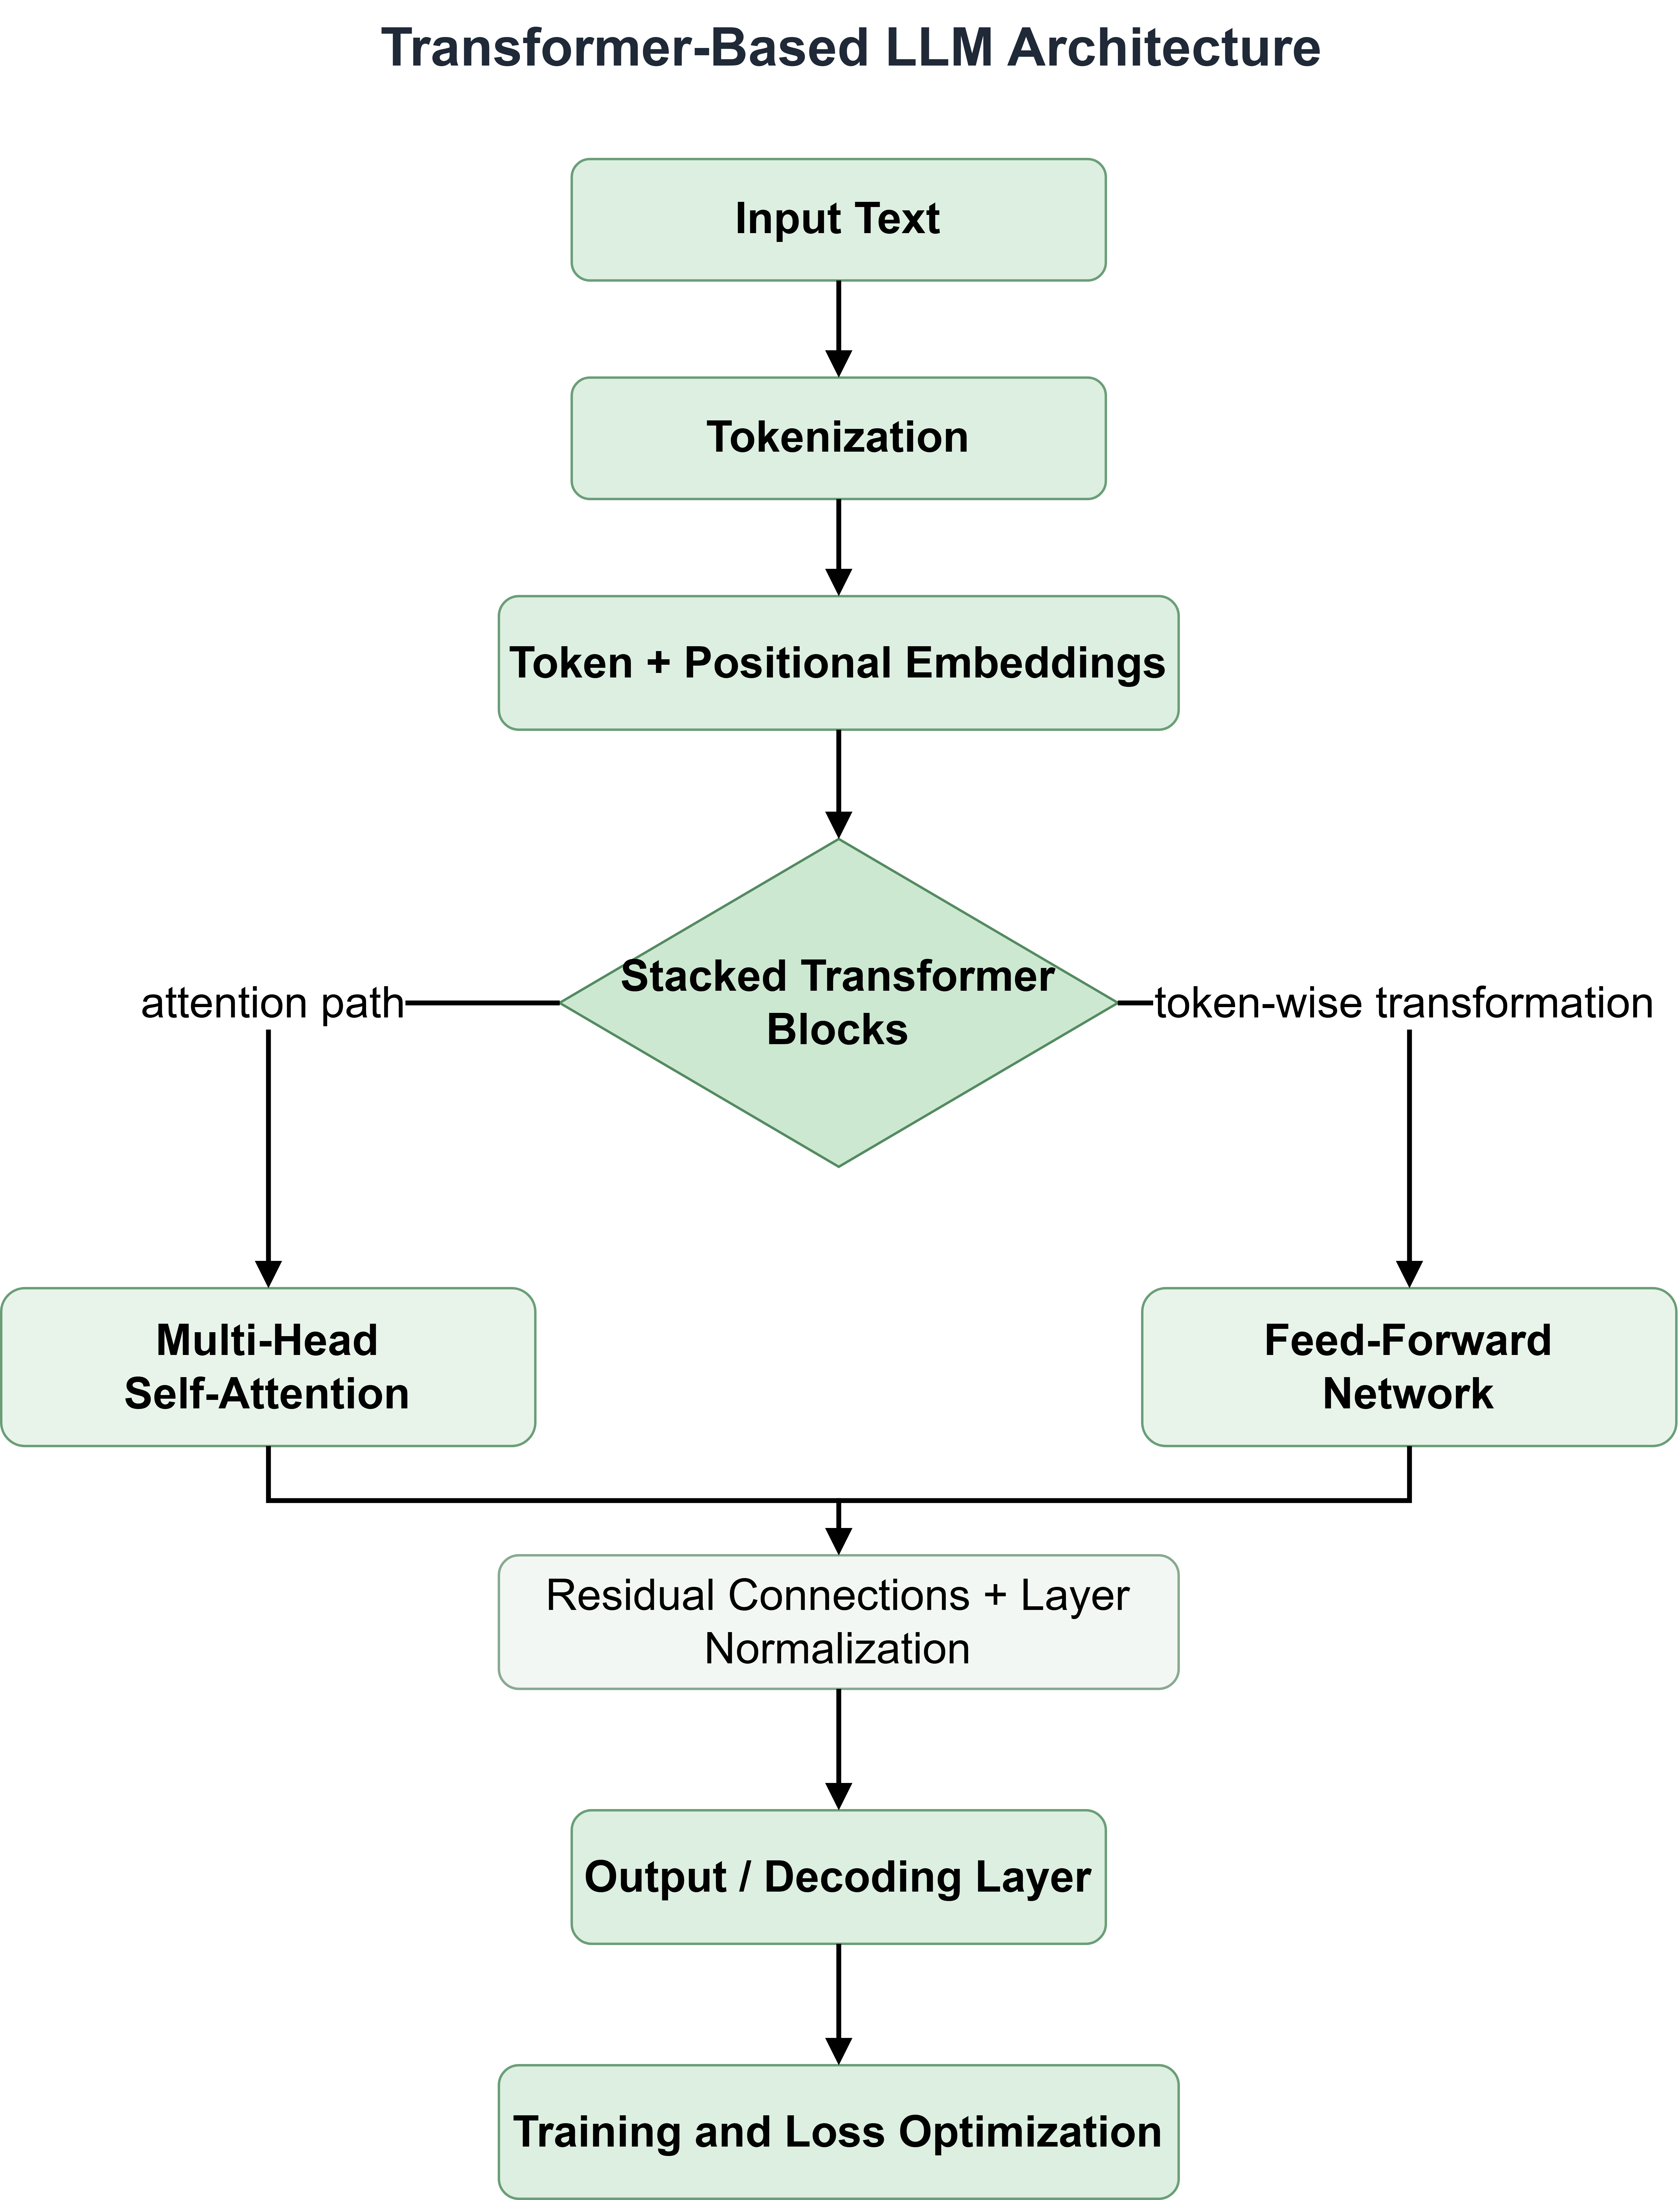
\includegraphics[width=0.78\textwidth,height=0.72\textheight,keepaspectratio]{images/llm_architecture.png}
    \caption{Simplified technical architecture of a Transformer-based large language model, adapted from \cite{gfg-llm-architecture}.}
    \label{fig:llm-architecture}
\end{figure}

Proprietary models may offer strong reasoning but raise privacy and sovereignty concerns, while open-weight models reduce vendor dependence at the cost of local computing requirements. LLMs also require substantial training data and computation, can inherit biases from their source corpora, and may generate unsupported information. These limitations justify grounding generation in retrieved documents, graph facts, and explicit citations \cite{lewis-rag}.

\subsection{Retrieval-Augmented Generation (RAG)}

Retrieval-Augmented Generation (RAG) augments LLM generation with dynamically retrieved external knowledge \cite{lewis-rag}. The classical pipeline indexes documents by chunking and embedding them, retrieves the top-$k$ relevant passages for a query, and conditions answer generation on that evidence. This workflow is efficient for direct factual questions but structurally limited for relational political analysis.

Recent extensions focus on \textbf{evidence grounding and citation}: retrieved passages are linked to sources, incomplete evidence triggers additional retrieval, and confidence checks reduce unsupported synthesis. These mechanisms do not replace RAG; they make generation auditable, which is essential when answers may influence interpretation of institutions, actors, or conflicts. Grounding also prepares the transition to graph-backed retrieval, where evidence includes explicit relations rather than isolated text spans.

\begin{figure}[H]
    \centering
    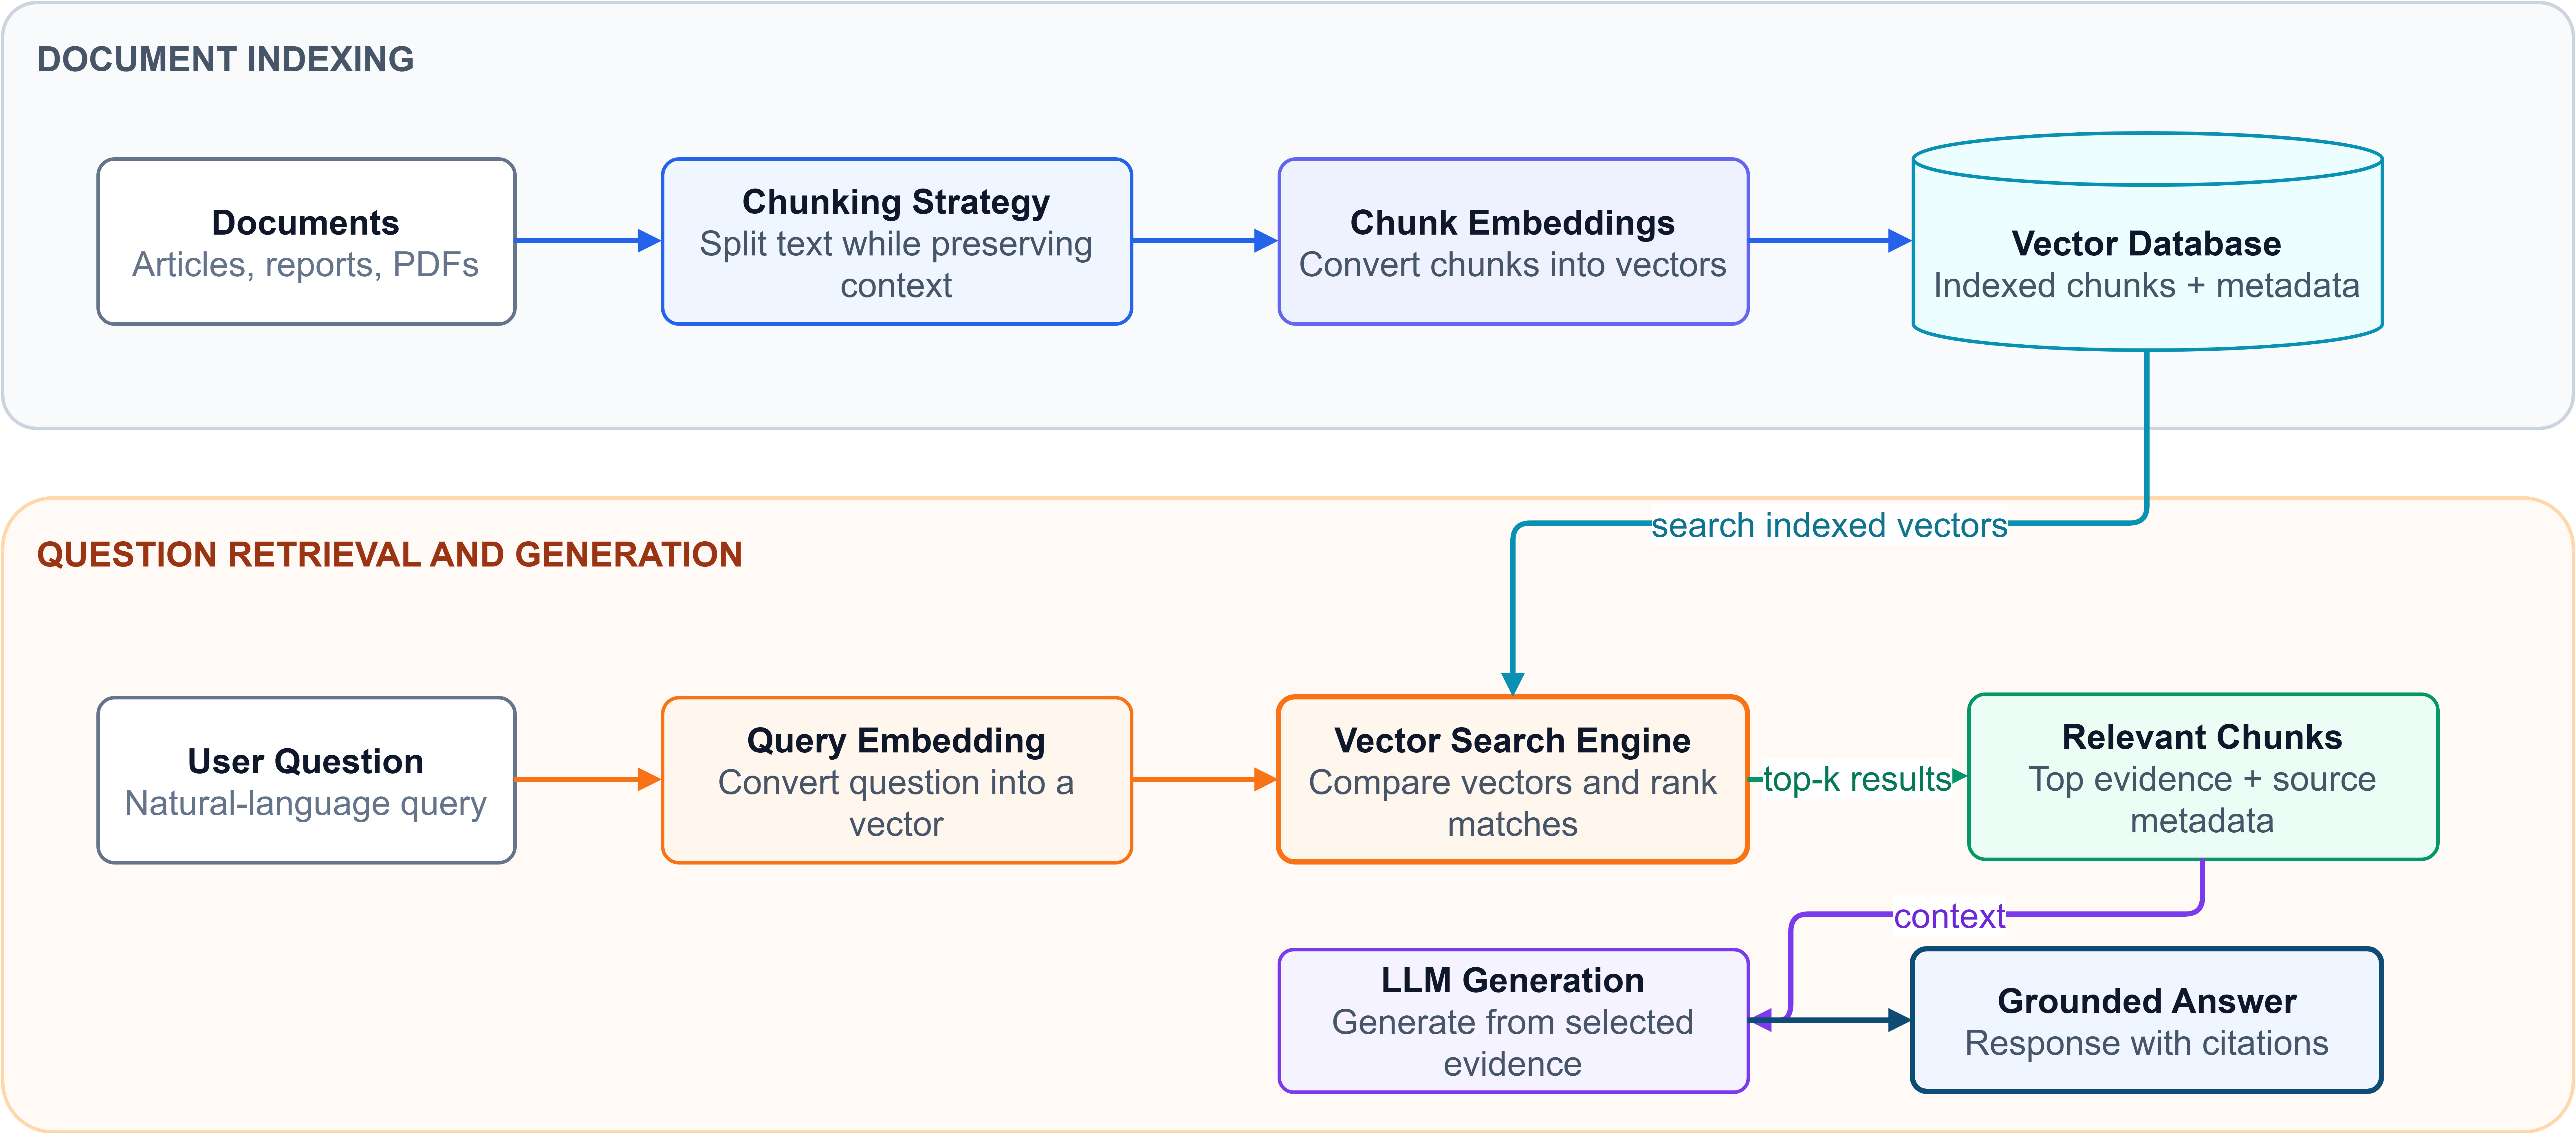
\includegraphics[width=0.92\textwidth,height=0.66\textheight,keepaspectratio]{images/rag_core_components.png}
    \caption{Core stages of a retrieval-augmented generation pipeline: indexing, retrieval, context construction, and grounded generation.}
    \label{fig:rag-core-components}
\end{figure}

Figure~\ref{fig:rag-core-components} separates the offline and online responsibilities of RAG. During indexing, source documents are parsed, divided into retrievable units, embedded, and stored with metadata. During querying, the user question is encoded, relevant evidence is selected, and the resulting context is supplied to the language model. The quality of the final answer therefore depends on each upstream stage rather than on generation alone.

\subsubsection{Chunking Strategies}

\noindent\textbf{Definition and role.} Chunking is the process of dividing a source document into smaller textual units before indexing. A RAG system generally does not embed an entire article or report as one vector because a long document may cover several topics and may exceed the context or input limits of the embedding model. Instead, each chunk becomes an independently searchable retrieval unit linked to its source document.

\par\smallskip\noindent
Chunk size directly affects retrieval behavior. Very small chunks can match a precise query but may omit the surrounding explanation needed to interpret the evidence. Very large chunks preserve context but can mix unrelated ideas, weaken similarity scores, consume more model context, and reduce the number of distinct sources that fit into one prompt. The objective is therefore not to maximize or minimize chunk length, but to preserve coherent evidence while keeping retrieval sufficiently precise.

\par\smallskip\noindent
\textbf{Main strategies.} Fixed-size chunking splits text after a predefined number of characters, words, or tokens. Overlapping chunking repeats part of the previous segment to reduce information loss at boundaries. Recursive chunking attempts progressively smaller separators, such as sections, paragraphs, sentences, and words. Structure-aware chunking follows document elements such as headings, paragraphs, lists, or pages. Semantic chunking groups neighboring sentences according to meaning rather than position alone. Table~\ref{tab:chunking-strategies} summarizes these alternatives.

\begin{table}[H]
\centering
\footnotesize
\setlength{\tabcolsep}{4pt}
\renewcommand{\arraystretch}{1.25}
\begin{tabularx}{\textwidth}{@{}>{\bfseries\raggedright\arraybackslash}p{2.5cm}>{\raggedright\arraybackslash}p{3.1cm}XX@{}}
\toprule
\rowcolor{lightblue}
Strategy & Principle & Main strengths & Main limitations \\
\midrule
Fixed-size & Split after a fixed number of characters, words, or tokens. & Simple, fast, predictable, and easy to reproduce. & Can cut sentences, arguments, dates, or relations at arbitrary boundaries. \\
Overlapping & Repeat a configurable portion of neighboring chunks. & Reduces boundary loss and preserves short-range continuity. & Creates duplicate content and increases index size and retrieval redundancy. \\
Recursive & Split by sections or paragraphs first, then use smaller separators when necessary. & Preserves natural text structure while respecting size limits. & Behavior depends on document formatting and separator quality. \\
Structure-aware & Use headings, paragraphs, lists, pages, or document markup as boundaries. & Produces interpretable chunks aligned with source organization. & Requires reliable parsing and varies across HTML, PDF, and other formats. \\
Semantic & Group sentences according to semantic similarity or topic shifts. & Better preserves coherent ideas and discourse units. & More computationally expensive and sensitive to the segmentation model. \\
\bottomrule
\end{tabularx}
\caption{Comparison of common chunking strategies in RAG systems \cite{gao-rag-survey,langchain-splitters,llamaindex-node-parsers}.}
\label{tab:chunking-strategies}
\end{table}

\textbf{Context expansion and project relevance.} Metadata should retain the source identifier, chunk position, section title, and links to adjacent chunks. A retrieval system can then search over compact units and selectively recover neighboring segments when a hit lacks sufficient context. This balances precision during initial retrieval with contextual completeness during answer synthesis. Chapter~4 describes the project-specific chunking configuration and adjacent-chunk expansion; the present discussion establishes the general design alternatives.

\subsubsection{Embedding Models}

\textbf{What is an embedding?} An embedding is a numerical vector that represents the semantic content of a text. An embedding model transforms both document chunks and user queries into vectors located in the same multidimensional space. Texts with similar meanings should be positioned closer together even when they use different vocabulary. A vector database can therefore retrieve a passage about diplomatic sanctions for a query that uses related wording without requiring an exact keyword match.

\textbf{Similarity search.} Retrieval commonly compares a query vector $\mathbf{q}$ with a document vector $\mathbf{d}$ using cosine similarity:
\[
\operatorname{cosine}(\mathbf{q},\mathbf{d})
=
\frac{\mathbf{q}\cdot\mathbf{d}}
{\lVert\mathbf{q}\rVert\,\lVert\mathbf{d}\rVert}.
\]
A higher score indicates a smaller angular distance and usually a stronger semantic match. The embedding model is therefore part of both indexing and querying: documents and questions must be encoded compatibly for their vectors to be meaningfully compared.

\textbf{Selection criteria.} Embedding models differ in vector dimension, language coverage, training data, inference cost, maximum input length, and domain specialization. Compact models reduce indexing time, storage, and query latency. Larger models may capture richer semantic distinctions but require more memory and computation. Multilingual models are important when the corpus contains English, French, Arabic, or transliterated names. Domain-specific models can improve specialized terminology, although they may generalize less effectively outside their training domain.

\begin{table}[H]
\centering
\footnotesize
\setlength{\tabcolsep}{4pt}
\renewcommand{\arraystretch}{1.25}
\begin{tabularx}{\textwidth}{@{}>{\raggedright\arraybackslash}p{3.35cm}>{\centering\arraybackslash}p{1.15cm}>{\raggedright\arraybackslash}p{2.05cm}XX@{}}
\toprule
\rowcolor{lightblue}
\textbf{Model} & \textbf{Dim.} & \textbf{Language scope} & \textbf{Main strengths} & \textbf{Main limitations} \\
\midrule
\texttt{all-MiniLM-}\newline\texttt{L6-v2} & 384 & Mainly English & Lightweight, fast, and economical for local indexing and baseline experiments. & Less suitable for multilingual corpora and subtle domain-specific distinctions. \\
\texttt{all-mpnet-}\newline\texttt{base-v2} & 768 & Mainly English & Richer semantic representation for general English retrieval. & Higher inference, memory, and vector-storage cost. \\
\texttt{paraphrase-}\newline\texttt{multilingual-}\newline\texttt{MiniLM-L12-v2} & 384 & Multilingual & Compact cross-language retrieval option covering English, French, and Arabic. & Multilingual breadth may reduce specialization for a particular domain. \\
Production-compatible\newline embedding service & Not disclosed & Multilingual & Integration with sovereign infrastructure and the deployed language-model ecosystem. & Exact model characteristics must be validated before scientific comparison. \\
\bottomrule
\end{tabularx}
\caption{Representative embedding-model alternatives and their principal retrieval trade-offs.}
\label{tab:state-of-art-embedding-models}
\end{table}

\textbf{Interpretation and project relevance.} Vector dimension alone does not determine retrieval quality. Chunk coherence, corpus language, metadata, query formulation, reranking, and the match between the model's training distribution and the target documents can outweigh a nominal increase in dimensionality \cite{gao-rag-survey}. Chapter~4 presents the embedding models considered during implementation and explains the transition from a compact baseline to a production-compatible multilingual service.

\subsubsection{Vector Databases for Semantic Retrieval}

Vector stores index dense representations and retrieve passages whose embeddings are close to the query even when their surface vocabulary differs. Their engineering differences concern more than raw search speed: persistence, metadata filtering, deployment complexity, distributed scaling, and integration with existing infrastructure all affect suitability for a RAG system. Table~\ref{tab:vector-store-comparison} compares representative options considered against the project's local-sovereignty and hybrid-retrieval requirements.

\begin{table}[H]
\centering
\footnotesize
\setlength{\tabcolsep}{4pt}
\renewcommand{\arraystretch}{1.25}
\begin{tabularx}{\textwidth}{@{}>{\bfseries\raggedright\arraybackslash}p{2.25cm}>{\raggedright\arraybackslash}p{2.45cm}XX@{}}
\toprule
\rowcolor{lightblue}
Tool & Type & Main strengths & Principal trade-offs \\
\midrule
FAISS & Similarity-search library & Mature CPU/GPU indexes for efficient dense-vector search and experimentation. & Persistence, metadata filtering, and service APIs must be engineered separately. \\
Qdrant & Vector database & Payload filtering, persistent collections, and REST/gRPC interfaces suited to production services. & Introduces an additional managed service and its operational footprint. \\
Weaviate & Vector database & Schema support, hybrid retrieval, filtering, and a broad semantic-search ecosystem. & A comparatively broad platform when only a compact local retrieval layer is required. \\
Milvus & Distributed vector database & Multiple ANN indexes, hardware-aware acceleration, and horizontal scaling for very large collections. & Distributed deployment and operations may be excessive for a focused end-of-study internship deployment. \\
Chroma & Embedded / client-server vector database & Accessible developer workflow for local prototypes and small RAG applications. & Fewer large-scale operational controls than distributed production-oriented systems. \\
Elasticsearch /\newline OpenSearch & Search platform with vector support & Combines lexical retrieval, filters, aggregations, and vector search in one search cluster. & Cluster administration and resource requirements are heavier than a dedicated local vector component. \\
ZVec & Local vector database & In-process persistence, metadata-linked chunk retrieval, and alignment with sovereignty constraints. & A smaller ecosystem and less operational maturity than long-established search platforms. \\
\bottomrule
\end{tabularx}
\caption{Comparison of representative vector-retrieval technologies \cite{faiss-docs,qdrant-docs,weaviate-docs,milvus-docs,chroma-docs,elasticsearch-vector-docs,opensearch-vector-docs,zvec-repo}.}
\label{tab:vector-store-comparison}
\end{table}

The comparison explains why no vector technology is universally preferable. FAISS is a strong algorithmic library but not a complete persistence service; Qdrant, Weaviate, Milvus, Elasticsearch, and OpenSearch provide richer service-level capabilities at the cost of additional deployment complexity; and Chroma emphasizes ease of prototyping. ZVec is relevant to the proposed architecture because semantic retrieval can remain local and lightweight while document provenance and explicit graph relations remain the responsibility of specialized stores. The implementation rationale is developed in Chapter~4.

\subsubsection{Hybrid Retrieval and Reranking}

\textbf{Definition and role.} Hybrid retrieval combines several evidence-selection mechanisms instead of relying on one similarity score. Dense retrieval identifies semantically related passages, lexical retrieval favors exact words and rare names, metadata filtering enforces constraints such as source, language, or date, and graph traversal recovers explicit relations between entities. Their candidate sets are fused before answer generation.

\textbf{Reranking.} The first retrieval stage is usually optimized for recall and returns a broader candidate set. A reranker then reorders or filters these candidates using stronger relevance signals. These may include semantic similarity, lexical overlap, graph distance, temporal validity, source quality, deduplication, or a cross-encoder that jointly reads the query and passage. Reranking improves precision but adds latency and requires calibration because scores from vector, lexical, and graph retrieval are not directly comparable.

\textbf{Project relevance.} Political questions frequently combine exact entities and dates with broader semantic intent. Hybrid retrieval is therefore better suited than a single search mechanism: lexical signals preserve precise names, vectors recover paraphrases, and graph paths expose multi-hop relations. RAG surveys treat query rewriting, filtering, reranking, and context assembly as central retrieval stages rather than optional post-processing \cite{gao-rag-survey}. The concrete fusion rules used by the platform are specified in Chapters~3 and~4.

\subsection{Information Extraction and Entity Resolution}

\textbf{Entity and relation extraction.} Knowledge construction begins by identifying entities, mentions, attributes, events, and relations in unstructured text. Rule-based approaches offer predictable behavior for stable patterns but require substantial maintenance when vocabulary or domains change. Supervised sequence-labeling and relation-classification models generalize better when annotated data are available, although separate extraction stages can propagate errors from entity detection to relation prediction. Transformer and LLM-based methods support joint or schema-guided extraction with less task-specific training data, but their outputs require structural validation because fluent generation does not guarantee factual or ontological correctness.

\begin{table}[H]
\centering
\footnotesize
\setlength{\tabcolsep}{4pt}
\renewcommand{\arraystretch}{1.25}
\begin{tabularx}{\textwidth}{@{}>{\bfseries\raggedright\arraybackslash}p{2.65cm}>{\raggedright\arraybackslash}p{3.1cm}XX@{}}
\toprule
\rowcolor{lightblue}
Approach & Principle & Strengths & Limitations \\
\midrule
Rule-based extraction & Handcrafted patterns, dictionaries, and grammatical rules identify entities and relations. & Predictable, interpretable, and effective for stable formats. & High maintenance cost and weak adaptation to new wording or domains. \\
Supervised pipelines & Trained models perform named-entity recognition followed by relation classification. & Measurable task performance and efficient inference after training. & Requires annotated data and can propagate errors between stages. \\
Joint transformer models & A shared encoder predicts entities and relations in one model. & Reduces pipeline fragmentation and captures contextual dependencies. & Still depends on domain-labeled data and predefined relation schemas. \\
LLM-based extraction & Prompted or fine-tuned LLMs generate schema-constrained structured records. & Flexible schemas, few-shot adaptation, and broad language understanding. & Higher cost, output variability, and risk of unsupported relations. \\
\bottomrule
\end{tabularx}
\caption{Comparison of representative entity and relation extraction approaches.}
\label{tab:extraction-approaches}
\end{table}

\textbf{Entity resolution.} Extracted mentions must be linked to canonical entities so that spelling variants, aliases, titles, and multilingual forms do not create fragmented graph nodes. Resolution may combine normalized names, contextual similarity, external identifiers, organizational roles, and temporal evidence. Deterministic rules improve reproducibility, while probabilistic or embedding-based methods improve recall on ambiguous mentions. In political corpora, the same surface name can refer to different people or institutions, and roles can change over time; resolution must therefore retain confidence, provenance, and the possibility of later correction.

\begin{table}[H]
\centering
\footnotesize
\setlength{\tabcolsep}{4pt}
\renewcommand{\arraystretch}{1.25}
\begin{tabularx}{\textwidth}{@{}>{\bfseries\raggedright\arraybackslash}p{2.7cm}>{\raggedright\arraybackslash}p{3.05cm}XX@{}}
\toprule
\rowcolor{lightblue}
Method & Evidence used & Strengths & Limitations \\
\midrule
Exact normalization & Case folding, punctuation removal, aliases, and normalized strings. & Fast, deterministic, and easy to audit. & Misses ambiguous, translated, or context-dependent mentions. \\
Knowledge-base linking & Candidate identifiers and descriptions from an external knowledge base. & Provides canonical identifiers and reusable background knowledge. & Coverage, update frequency, and external dependence may be limiting. \\
Contextual similarity & Mention context is compared with candidate descriptions or previous mentions. & Handles aliases and ambiguous surface forms more effectively. & Requires thresholds and may produce opaque similarity errors. \\
Hybrid resolution & Combines deterministic rules, context, metadata, and optional human review. & Balances reproducibility, recall, and correction mechanisms. & More complex to calibrate and maintain across domains. \\
\bottomrule
\end{tabularx}
\caption{Comparison of common entity-resolution strategies.}
\label{tab:entity-resolution-strategies}
\end{table}

\textbf{Graph quality and provenance.} Extraction confidence alone is insufficient for a trustworthy knowledge graph. Pipelines must detect duplicates, reject malformed relations, preserve source spans, and represent contradictory or temporally superseded claims without silently overwriting them. Provenance connects every node or relation to the document and passage from which it was derived. This evidence chain supports graph repair, analyst verification, and cited generation, while temporal metadata distinguishes a current fact from a historically valid one.

\subsection{Knowledge Graphs and Graph-RAG}

\textbf{Knowledge graph fundamentals.} A knowledge graph represents information as entities connected by typed relations. Entities become nodes, relations become edges, and both may carry properties such as names, dates, confidence values, source identifiers, or validity intervals. Unlike a flat document index, this representation makes relationships explicit and supports traversals such as identifying organizations connected to an actor through several intermediate events.

\begin{figure}[H]
    \centering
    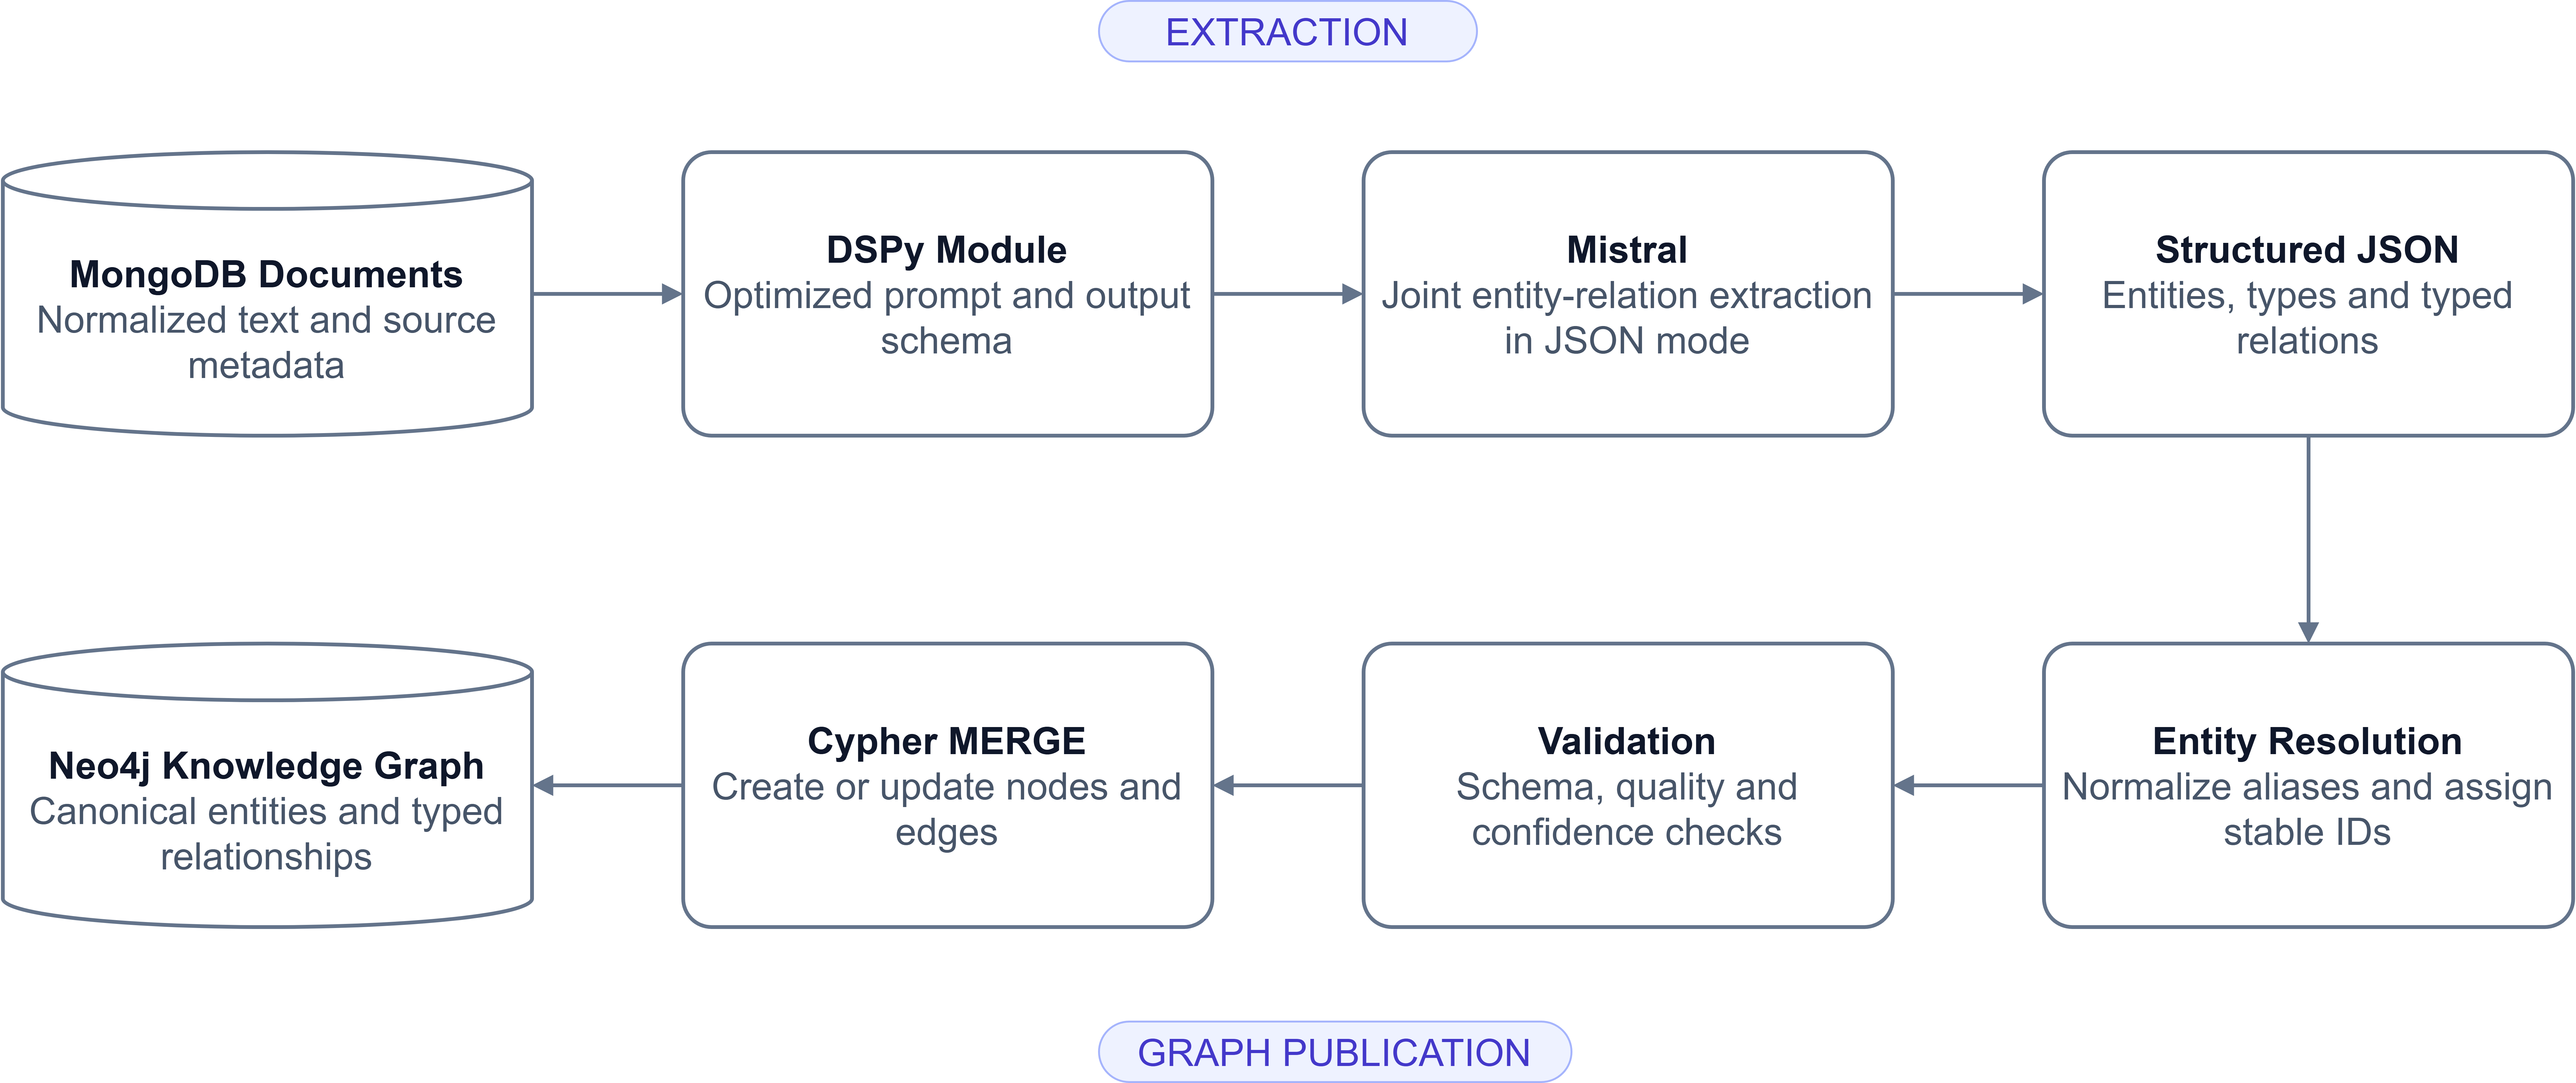
\includegraphics[width=0.88\textwidth,height=0.65\textheight,keepaspectratio]{images/knowledge_graph_construction.png}
    \caption{General process for constructing a knowledge graph from unstructured documents.}
    \label{fig:knowledge-graph-construction}
\end{figure}

As shown in Figure~\ref{fig:knowledge-graph-construction}, graph construction transforms documents into mentions, canonical entities, and validated relations before publication. An ontology or schema constrains the permitted entity and relation types, while provenance links the resulting facts back to their evidence. Graph queries can then filter by type, follow multi-hop paths, aggregate neighborhoods, and reason over temporal or organizational structures.

Classical RAG retrieves passages through semantic similarity. Graph-RAG constructs or uses graph-structured knowledge and retrieves through entities, relationships, communities, and source passages \cite{edge-graphrag,microsoft-graphrag}. Figure~\ref{fig:rag-vs-graphrag} contrasts the two retrieval paths and shows why geopolitical questions often require relational traversal.

\begin{figure}[H]
    \centering
    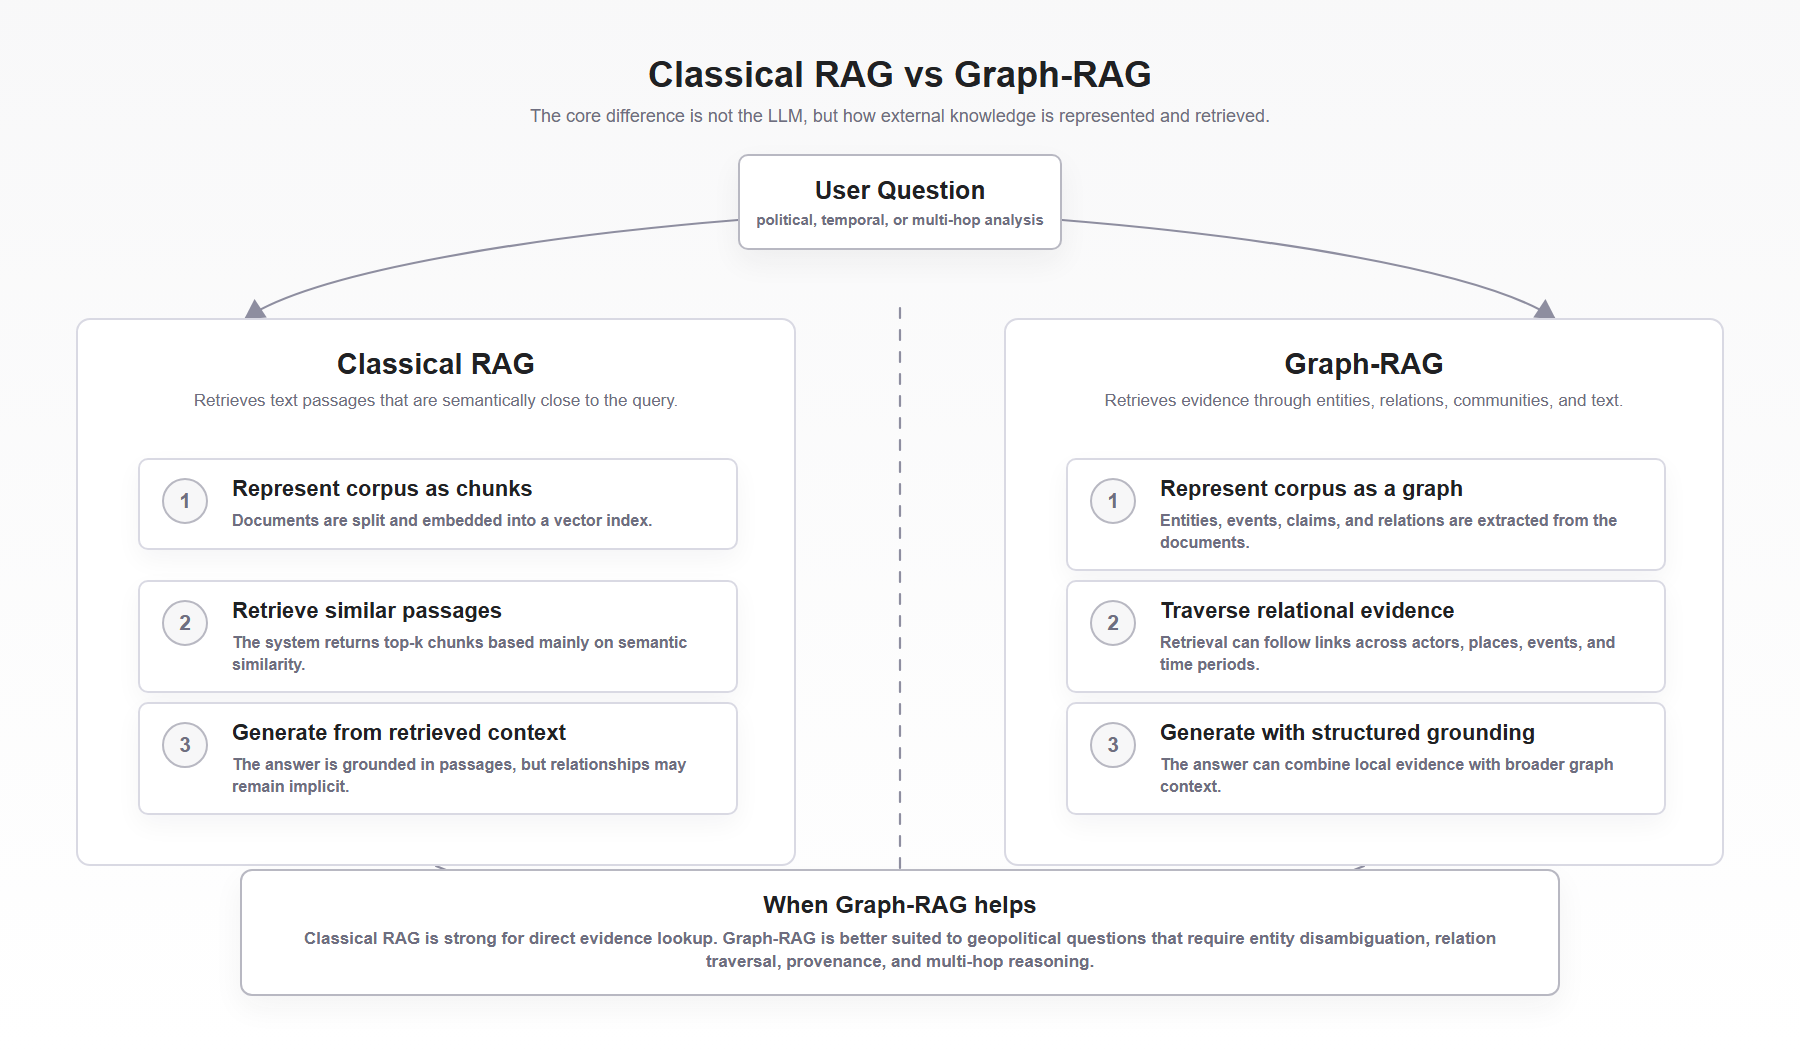
\includegraphics[width=\textwidth,height=0.82\textheight,keepaspectratio]{images/rag_vs_graphrag.png}
    \caption{Comparison between classical RAG and Graph-RAG retrieval paths.}
    \label{fig:rag-vs-graphrag}
\end{figure}

\textbf{Knowledge graph concepts.} A knowledge graph represents entities and typed relations, optionally with temporal or provenance metadata. It supports entity disambiguation, path queries, and hybrid retrieval that combines vector similarity with structural constraints.

\textbf{Graph construction from text.} Pipelines typically perform extraction, entity resolution, and provenance linking so that each relation remains traceable to a source document. Noise control is critical because LLM-based extraction can introduce spurious nodes or edges if resolution rules are weak.

\textbf{Graph-RAG retrieval and reasoning.} Once published, the graph enables multi-hop traversal, community summarization, and fusion with textual chunks retrieved by dense search \cite{edge-graphrag,microsoft-graphrag}. This combination is particularly relevant when answers depend on chains of actors and events rather than on a single paragraph.

\begin{table}[H]
\centering
\footnotesize
\setlength{\tabcolsep}{4pt}
\renewcommand{\arraystretch}{1.25}
\begin{tabularx}{\textwidth}{@{}>{\bfseries\raggedright\arraybackslash}p{2.7cm}>{\raggedright\arraybackslash}p{3.1cm}XX@{}}
\toprule
\rowcolor{lightblue}
Strategy & Retrieval focus & Strengths & Limitations \\
\midrule
Local Graph-RAG & Entity neighborhoods and short paths around query-linked nodes. & Precise evidence for entity-centric and multi-hop questions. & Can miss corpus-wide themes or disconnected relevant evidence. \\
Global and community Graph-RAG & Community summaries and hierarchical graph themes. & Supports broad questions requiring corpus-level synthesis \cite{edge-graphrag}. & Summary construction is costly and may hide minority evidence. \\
Hybrid Graph-RAG & Dense chunks are fused with graph nodes, paths, or communities. & Combines semantic recall with relational precision and provenance. & Requires score calibration, deduplication, and more complex orchestration. \\
Agentic Graph-RAG & A controller iteratively selects graph, vector, or external tools. & Adapts retrieval depth and tool choice to question complexity. & Higher latency, cost, and risk of unstable tool-selection loops. \\
\bottomrule
\end{tabularx}
\caption{Comparison of representative Graph-RAG retrieval strategies.}
\label{tab:graphrag-strategies}
\end{table}

\textbf{Limitations of Graph-RAG.} Graph-RAG transfers part of the retrieval problem into graph construction and maintenance. Extraction errors can create incorrect paths, entity-resolution errors can merge unrelated actors or fragment one actor across nodes, and community summaries can hide minority or contradictory evidence. Graph construction also adds computational cost, storage, update logic, and ontology-management effort. As the source corpus evolves, stale relations and summaries must be refreshed while provenance and temporal validity remain intact. Graph-RAG is therefore most useful when relational retrieval justifies this additional complexity and when graph evidence remains connected to inspectable source passages.

\subsection{LLM Reasoning and Thinking Modes}

Beyond retrieval format, recent work studies how a language model \emph{uses} evidence during generation. Classical RAG follows a mostly linear pipeline: retrieve once, then generate. This design is efficient for localized factual questions, but it is structurally weak when a query requires several retrieval steps, intermediate planning, or verification of partial evidence \cite{lewis-rag}.

\textbf{Chain-of-Thought and query decomposition.} Chain-of-Thought (CoT) prompting asks the model to produce intermediate reasoning steps before the final answer \cite{wei-cot}. In retrieval settings, decomposition splits a complex question into sub-questions and guides evidence collection step by step. The goal is not longer answers for their own sake, but better coverage when the first retrieved batch is incomplete.

\textbf{Interleaved retrieval and multi-hop reasoning.} IRCoT interleaves retrieval with ongoing chain-of-thought generation: each reasoning step can trigger a new retrieval call guided by what was learned in the previous step \cite{trivedi-ircot}. This pattern is especially relevant for multi-hop questions where bridge entities only become visible after an initial pass. When knowledge is graph-structured, multi-hop traversal plays a similar role by following explicit paths between actors and events rather than relying on lexical similarity alone.

\textbf{ReAct and tool-interleaved control.} ReAct combines reasoning traces with actions such as search, graph lookup, or tool invocation \cite{yao-react}. Instead of a fixed retrieve-then-generate sequence, the model alternates between thinking steps and operations on external memory. This architecture is a precursor to modern agentic pipelines in which a controller decides when to retrieve again, when to stop, and when to synthesize.

\textbf{Reflection and Self-RAG.} Reflection-based methods add a critique step that evaluates whether the current evidence supports the draft answer. Self-RAG trains the model to decide when retrieval is needed, when generation is sufficient, and when the output should be revised \cite{asai-selfrag}. These approaches reduce unsupported synthesis at the cost of additional model calls and higher latency.

\textbf{Agentic RAG.} Agentic RAG generalizes the above patterns into loops that may include planning, routing, iterative retrieval, critique, and final synthesis. Surveys of the field describe a recurring trade-off: iterative and reflective pipelines improve faithfulness on relational or multi-step tasks, but they increase token cost and response time compared with naive RAG. For political intelligence, this literature motivates architectures in which reasoning depth can be adapted to question complexity rather than forcing every query through the heaviest pipeline.

\begin{table}[H]
\centering
\footnotesize
\setlength{\tabcolsep}{4pt}
\renewcommand{\arraystretch}{1.25}
\begin{tabularx}{\textwidth}{@{}>{\bfseries\raggedright\arraybackslash}p{2.2cm}>{\raggedright\arraybackslash}p{3.0cm}XX@{}}
\toprule
\rowcolor{lightblue}
Method & Core mechanism & Main benefit & Main trade-off \\
\midrule
Chain-of-Thought & Generates intermediate reasoning steps before answering \cite{wei-cot}. & Improves decomposition of complex questions. & Reasoning can remain disconnected from new evidence retrieval. \\
IRCoT & Alternates reasoning steps with additional retrieval \cite{trivedi-ircot}. & Recovers bridge evidence for multi-hop questions. & Requires several retrieval and generation cycles. \\
ReAct & Interleaves reasoning with explicit tool actions \cite{yao-react}. & Supports search, graph lookup, and observable actions. & Tool-selection errors can propagate through the trajectory. \\
Self-RAG & Reflects on retrieval need, evidence quality, and generated output \cite{asai-selfrag}. & Improves evidence sufficiency and self-correction. & Adds model calls, training complexity, and latency. \\
Agentic RAG & Plans, routes, retrieves, critiques, and stops dynamically. & Adapts reasoning depth to the task and available tools. & Highest orchestration complexity and operational cost. \\
\bottomrule
\end{tabularx}
\caption{Comparison of reasoning and control strategies used in retrieval-augmented systems.}
\label{tab:reasoning-strategies}
\end{table}

Chapter~4 presents the reasoning modes implemented in the platform and describes how these ideas are operationalized in production.

\subsection{Political NLP and Temporal Modeling}

Political NLP extends language understanding to actors, institutions, stances, conflicts, and temporal relations. Joint entity-and-relation extraction reduces error propagation, stance analysis identifies how actors relate to events or entities \cite{allaway-stance}, and temporal knowledge graphs attach validity intervals to evolving facts \cite{trivedi-hyte}. These capabilities explain why political intelligence requires extraction, temporal modeling, and retrieval rather than a single summarization model.

Political text also presents domain-specific ambiguity. Statements may report allegations rather than established facts, sources may express conflicting positions, and institutional roles may change while names remain constant. Systems must distinguish the author of a claim from the actor described by it, preserve publication dates separately from event dates, and avoid treating repeated syndicated reports as independent confirmation. Multilingual coverage further complicates entity aliases, transliteration, and stance interpretation across English, French, and Arabic sources.

\subsection{Evaluation of Retrieval-Augmented Systems}

RAG evaluation must distinguish retrieval failure from generation failure. Retrieval-oriented measures examine whether relevant evidence was returned, commonly through precision, recall, or ranked-relevance analysis. Generation-oriented measures assess whether the answer addresses the question, remains supported by the retrieved context, and correctly reflects a reference answer. Citation evaluation adds another layer by checking whether cited passages actually support the claims attributed to them.

RAGAS formalizes this multidimensional view through metrics such as faithfulness, answer relevancy, context precision, context recall, and answer correctness \cite{ragas-paper,ragas-answer-correctness}. These measures are useful because a fluent answer can still be unsupported, while a weak final answer may originate from insufficient retrieval rather than from the generator itself. Automatic LLM-based judges make repeated evaluation practical but introduce model bias and should be complemented by transparent benchmark construction, error analysis, and human review for high-stakes domains.

For Graph-RAG, evaluation should additionally test multi-hop coverage, entity resolution, path validity, provenance completeness, temporal consistency, and the cost-latency trade-off of iterative reasoning. A system may improve relational answer quality while increasing response time or model calls; reporting only final-answer accuracy would hide this operational trade-off.

\subsection{Related Systems and Gap Analysis}

Representative systems illustrate how these approach families are realized in practice. The original RAG architecture combines dense retrieval with sequence generation for knowledge-intensive NLP tasks \cite{lewis-rag}. Microsoft GraphRAG organizes extracted entities into communities and produces hierarchical summaries for local and global questions \cite{edge-graphrag,microsoft-graphrag}. Wikidata provides a collaboratively maintained structured knowledge graph with SPARQL access \cite{wikidata-sparql}. GDELT continuously monitors global news and publishes event-oriented structured data, including its Global Knowledge Graph \cite{gdelt-official,gdelt-gkg}. These systems solve complementary parts of the problem, but none directly provides the complete combination of domain-adaptable extraction, local hybrid retrieval, selectable reasoning depth, analyst-facing evidence, and supervised ingestion targeted by this project.

Table~\ref{tab:comparative-summary} compares the corresponding approach families along criteria relevant to political intelligence. The comparison does not claim that one row is universally superior; it reveals structural trade-offs that motivate the platform studied during this end-of-study internship.

\begin{table}[H]
\centering
\footnotesize
\setlength{\tabcolsep}{4pt}
\renewcommand{\arraystretch}{1.25}
\begin{tabularx}{\textwidth}{@{}>{\bfseries\raggedright\arraybackslash}p{3.2cm}>{\centering\arraybackslash}X>{\centering\arraybackslash}X>{\centering\arraybackslash}X>{\centering\arraybackslash}X@{}}
\toprule
\rowcolor{lightblue}
Criterion & Classical RAG & MS GraphRAG & Knowledge Graph & Agentic RAG \\
\midrule
Multi-hop reasoning & Limited & Yes & Yes & Yes \\
Entity disambiguation & Limited & Yes & Yes & Depends on tools \\
Temporal reasoning & No & Partial & Yes & Partial \\
Source citation & Yes & Yes & Partial & Yes \\
Structured queries & No & Limited & Yes & Depends on tools \\
Explicit provenance & Passage level & Passage and graph & Fact level & Tool dependent \\
Multilingual support & Model dependent & Model dependent & Schema dependent & Model dependent \\
Adaptive reasoning & No & Limited & No & Yes \\
Autonomous ingestion & External pipeline & External pipeline & External pipeline & Possible \\
\bottomrule
\end{tabularx}
\caption{Comparative summary of major approach families across retrieval, reasoning, and evidence-management criteria.}
\label{tab:comparative-summary}
\end{table}

Classical RAG supports passage-level citation but lacks explicit multi-hop and temporal modeling. Microsoft GraphRAG improves structured retrieval and graph-backed summarization but assumes that ingestion and graph maintenance are handled by surrounding processes. Pure knowledge graphs excel at structured, provenance-aware, and temporal queries but do not, by themselves, provide conversational synthesis. Agentic RAG adapts retrieval actions to the question but depends strongly on the quality of its tools and can increase latency and cost. No approach family satisfies every criterion by default; the remaining challenge is to integrate ingestion, hybrid retrieval, graph reasoning, provenance, and grounded generation in one auditable workflow.

\section{Research Gap and Positioning}
\label{sec:research-gap-positioning}

The central research gap is the inability of classical retrieval systems to represent political information as evolving relational structures. Semantic search can surface topically similar documents, but it does not explicitly model who is connected to whom, through which event, under which institutional role, and during which temporal interval.

The platform developed during the internship addresses this gap through a hybrid architecture. Dense vector retrieval contributes semantic recall over unstructured documents, while the knowledge graph contributes relational precision, entity disambiguation, and multi-hop traversal. Compared with Table~\ref{tab:comparative-summary}, the contribution of this end-of-study internship does not claim universal superiority on every criterion; rather, it targets an integrated combination that was missing in the compared families:

\begin{itemize}[leftmargin=*, itemsep=4pt]
\item \textbf{Hybrid evidence:} joint use of vector chunks, graph relations, and document provenance in the same query workflow.
\item \textbf{Supervised ingestion:} autonomous collection with operational control, rather than a static benchmark corpus only.
\item \textbf{Selectable reasoning depth:} one-hop, decomposed multi-hop, and reflexive modes to trade latency against analytical coverage (Chapter~4).
\item \textbf{Remaining limits:} semantic deduplication, full temporal normalization, and large-scale multilingual coverage are still partial and are discussed in Chapter~5.
\end{itemize}

From this perspective, the project contributes along three axes:

\begin{itemize}[leftmargin=*, itemsep=4pt]
\item \textbf{Methodological contribution:} studying how graph-structured evidence improves faithfulness, explainability, and temporal consistency of LLM-based political analysis.
\item \textbf{Technical contribution:} combining ingestion, hybrid retrieval, graph publication, and reasoning modes in one platform grounded in provenance.
\item \textbf{Operational contribution:} delivering an end-to-end workflow in which analysts query evidence, inspect sources, explore graph neighborhoods, and supervise ingestion without modifying backend code.
\end{itemize}

In functional terms, the system is a reasoning multimodal Graph-RAG platform: it collects heterogeneous political documents, converts them into chunks and graph relations, retrieves evidence through vector and graph stores, and produces cited answers through an LLM orchestration layer (Mistral with DSPy modules, as detailed in Chapter~4). This gap therefore corresponds to a concrete need observed during the internship: analysts require continuous ingestion, structured knowledge, semantic retrieval, and explainable generation in a single environment.

\section{Conclusion}

This chapter reviewed the state of the art required to position the proposed Graph-RAG framework. It covered large language models, RAG, chunking, embeddings, vector retrieval, information extraction, entity resolution, knowledge graphs, Graph-RAG, reasoning paradigms, political NLP, temporal modeling, and evaluation methods. The comparison showed that classical RAG, graph-based retrieval, knowledge graphs, and agentic approaches provide complementary capabilities but do not jointly guarantee autonomous ingestion, provenance, multilingual coverage, adaptive reasoning, and auditable synthesis. These limitations define the research position of the proposed hybrid framework. Chapter~3 translates the requirements established in Chapter~1 and the scientific foundations reviewed here into the system design and architecture.

